\chapter{Theoretical Analysis} \label{chap:det-theory}

In this chapter we show the reader that MongoDB cannot always guarantee write durability. We do so by establishing the conditions required for a write to be lost, using a theoretical approach based on the the background information of how MongoDB processes and persists write operations. We conclude with a categorisation of MongoDB's write durability failures in terms of these conditions. This theory will then motivate the measurements described in \prettyref{chap:experiments} to help users evaluate the risk of lost writes.

\section{Introduction}
Recall from \prettyref{chap:background} that MongoDB replication scheme works in a primary-secondary configuration. That is, a single primary node is elected and becomes the \textit{arbiter of all write operations}. This means that the primary will receive all write operations before informing the secondary nodes of the operations' existence. From this we can intuitively conclude that a crash can result in a lost write if that write has been acknowledged by the primary but has not been persisted to disk.

However, MongoDB replica sets also support elections when a primary crashes, in order to elect a new primary and minimise downtime. This creates a situation where a secondary can get promoted to the role of a primary without having received all operations from the crashed primary. In these circumstances, when the crashed node goes back online, it must \textit{roll back} any operations that it acknowledged but are not on the new primary. This can directly result in writes being lost despite being acknowledged and persisted.

\section{Write Loss}
Recall that, in a durable system, all acknowledged writes must remain committed even in case of system failure. As such, it is a violation of durability if an acknowledged write is not reflected in the reads following the acknowledgement. Therefore, we define a write as lost when a read on the document returns a version older than the latest acknowledged write. An example of this can be seen in \prettyref{fig:wl}.

\begin{figure}
    \begin{CVerbatim}
write x = 1
ack   x = 1
...
read  x -> x = 0
    \end{CVerbatim}
    \caption{Sample scenario depicting write loss}
    \label{fig:wl}
\end{figure}

We observe that a write loss may be permanent or it may merely be transient. Permanent write loss involves an acknowledged write being erased or rolled back such that its effects are completely removed from the data and \textit{all} subsequent reads return a version older than the lost write. On the other hand, a transient write loss involves a read returning an older version temporarily, with the latest version of the document eventually being returned.

\section{Write Loss Scenarios}
On the assumption that the only way a machine could fail is to crash, the conditions for permanently losing an acknowledged write will fall broadly into two categories:
\begin{enumerate}
    \item Rollback due to re-election
    \item Primary crashed before persisting
\end{enumerate}

Observe that category 1 losses are a direct consequence of how long it takes for the node to receive a write while  category 2 losses are related to the time it takes to make the write durable. 

We also find that a transient write loss can occur if the client's read preference is configured as "Primary Preferred".

We now present each of these scenarios in detail.

\pagebreak
\subsection{Rollback due to re-election}
\begin{figure}[H]
    \centering
    \includegraphics{images/reelection.pdf}
    \label{fig:reelection}
    \caption{A time-space diagram of a scenario where a write gets lost due to a re-election}
\end{figure}

We define the entire sequence of operations currently in the primary's Oplog as $O$. This failure is induced when the replica set notices that the primary node ($p$) has crashed. At this point, it is possible that \textit{none} of the secondaries managed to read the entire Oplog. This results in the existence of a sequence of one or more operations that have been committed to the primary but left completely unknown to the rest of the replica set. For MongoDB, this sequence \textit{must} be a suffix of $O$ (see \prettyref{sec:replication}), which we will denote as $\hat{O}$.

Upon a re-election, the replicas will announce the last operation they applied ($o$). MongoDB's election procedure will elect the primary, such that it minimises the size of $\hat{O}$, however since there are \textit{some} operations have have been seen by \textit{none} of the replicas, $|\hat{O}| > 0$ must hold. 

After being elected, the new primary ($p'$) will establish its Oplog as the source of truth. This Oplog will contain operations $O - \hat{O}$. When the original node $p$ goes back online, it still has the operations applied as per Oplog $O$. Since $p$ is no longer the primary, it must synchronize its state with $p'$, which will involve \textit{rolling back} all operations in $\hat{O}$. This is precisely the loss of writes as a result of a rollback.

As such, this failure scenario can occur with primary write concern and journaled, but it will not occur (in a properly implemented MongoDB system) with write concern majority.

\pagebreak
\subsection{Crash before persisting}
\begin{figure}[H]
    \centering
    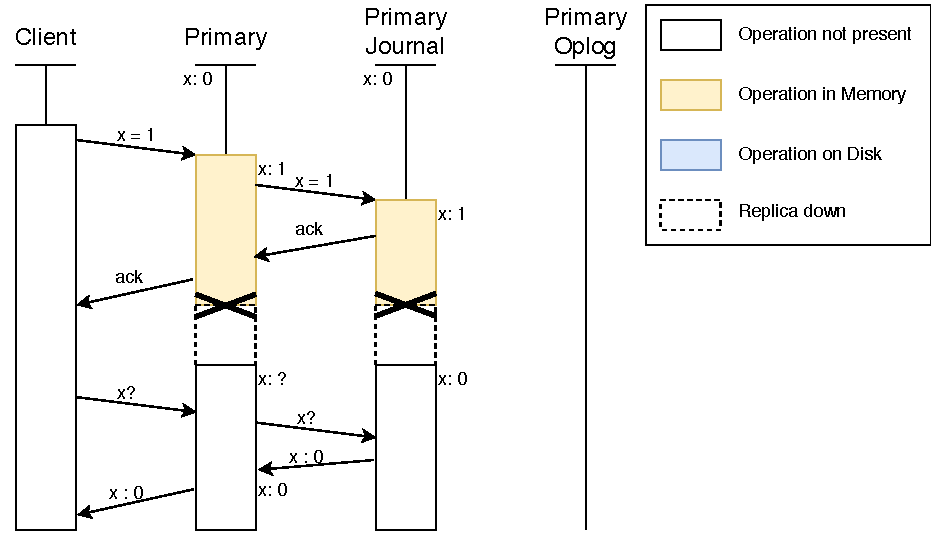
\includegraphics{images/nopersist.pdf}
    \label{fig:nopersist}
    \caption{A time-space diagram of a scenario where a write gets lost due to a failure to persist it on disk}
\end{figure}

This failure relies on two core properties of MongoDB - acknowledging a write before persisting it and only adding a write to the Oplog after flushing it to disk.

Take an operation $o$, with write concern \textit{journaled}, which has just been received by the primary. Currently, the primary stores this operation in memory, performs the operation on the in-memory copy of the data and buffers the write to the journal, but does not yet flush it to disk. Recall that a write is added to the Oplog only \textit{after} it has been flushed to disk. This creates a situation where secondary nodes do not know about a write that has been acknowledged by the primary. As such, if a primary is to crash it will "forget" about $o$ as it was only stored in memory. None of the secondary replicas would have seen $o$ either. A client querying the primary will force it to read the last value of the document operated on from disk. The value returned from the read will not account for the latest operation, which demonstrates the operation has been lost.

Thus, this failure scenario occurs with primary write concern but may also occur with journaled, if the write is buffered instead of being immediately persisted. It will not occur (in a properly implemented MongoDB system) with write concern majority.

\pagebreak
\subsection{Transient Loss via Primary Preferred Read Preference}
\begin{figure}[H]
    \centering
    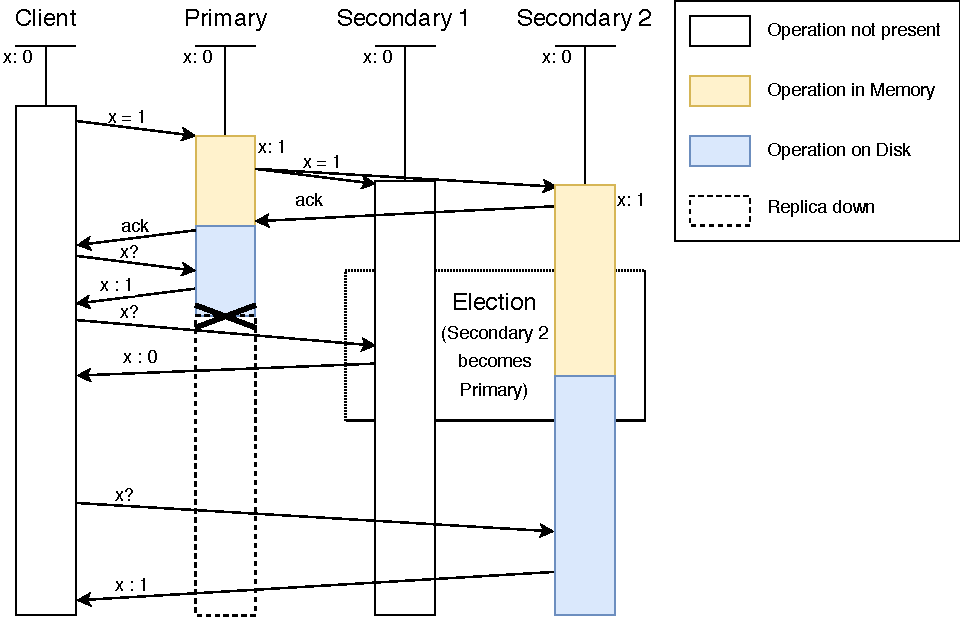
\includegraphics{images/PrimaryPreferred.pdf}
    \label{fig:primarypreferred}
    \caption{A time-space diagram of a scenario where a Majority write concern write gets temporarily lost as a result of the MongoDB client choosing the wrong Secondary to read from.}
\end{figure}

Recall from \prettyref{sec:readpref} that the Primary Preferred read preference will query the secondary if the primary appears to be down, instead of waiting for a primary to respond. The MongoDB client will only query one secondary. This can create a situation where a write will seem to be available, lost and available again. 

Specifically, consider an operation $o$ that was submitted with a majority write concern to the replica set. The primary will acknowledge the write when $\lfloor\frac{|R|}{2}\rfloor$ secondaries also acknowledge the write. This leaves $\lfloor\frac{|R|}{2}\rfloor$ secondaries that may not have acknowledged or even received the write. As such, if the primary is to fail immediately after acknowledging the operation, the MongoDB client has $\frac{\lfloor\frac{|R|}{2}\rfloor - 1}{|R|}$ chance of querying  a secondary that has not seen $o$. Intuitively, this probability reduces with time as more replicas apply the operation to their copy of the data.

If the client is to query the primary, the data returned will have operation $o$ applied to it. Once the primary fails, the MongoDB client has a chance of querying a secondary that has not applied the operation, hence the data returned from that query will not have the operation $o$ applied. Querying the new primary after an election will once again return data with operation $o$ applied. 

As such, Primary Preferred read preference can create instances of transient write loss, where acknowledged operations seem to disappear and reappear during a failure. This scenario can occur in all write concerns, but "all".